\documentclass[12pt,spanish]{article}

\usepackage[left=2.5cm,right=2cm,top=2cm,bottom=2cm]{geometry}
\setlength{\parindent}{0mm}

\usepackage{float}

\usepackage{parskip}
\usepackage[document]{ragged2e}
\usepackage{babel}
\usepackage[utf8]{inputenc}
\usepackage{amsmath,amsthm,mathtools}
\usepackage{amsfonts,amssymb,latexsym}
\usepackage{enumerate}
\usepackage[dvips,usenames]{color}
\definecolor{RojoAnayelRey}{rgb}{1,.25,.25}
\usepackage{tikz}
\usepackage[bookmarks=true,
bookmarksnumbered=false, % true means bookmarks in 
% left window are numbered                         
bookmarksopen=false,     % true means only level 1
% are displayed.
colorlinks=true,
linkcolor=blue]{hyperref}

\usepackage{beton}
\usepackage[T1]{fontenc}

% Theorem environments

%% \theoremstyle{plain} %% This is the default
\newtheorem{theorem}{Teorema}[section]
\newtheorem{corollary}[theorem]{Corolario}
\newtheorem{lemma}[theorem]{Lema}
\newtheorem{proposition}[theorem]{Proposici\'on}
% \newtheorem{ax}{Axioma}

\theoremstyle{definition}
\newtheorem{definition}{Definici\'on}[section]
\newtheorem{algorithm}{\textrm{\bf Algoritmo}}[section]

\theoremstyle{remark}
\newtheorem{remark}{Observaci\'on}
\newtheorem{example}{Ejemplo}
\newtheorem{exercise}{Ejercicio}
% \newenvironment{solution}{\begin{proof}[Solution]}{\end{proof}}
\newenvironment{solution}{\begin{proof}
    [Solución]}{\end{proof}}
\newtheorem*{notation}{Notaci\'on}

\newcommand{\R}{\mathbb{R}}

\renewcommand\labelenumi{(\roman{enumi})}
\renewcommand\theenumi{\labelenumi}

\title{Mecánica Celeste: Problemas Tema 1}

\author{David Cabezas Berrido}

\date{}

\begin{document}
\maketitle

\newcommand{\ch}{\operatorname{ch}}
\newcommand{\sh}{\operatorname{sh}}
\newcommand{\ach}{\operatorname{arc}\ch}
\newcommand{\ash}{\operatorname{arc}\sh}

\setcounter{exercise}{4}
\begin{exercise}
  \begin{align*}
    \Phi : \R\times \mathbb{R}^+&\rightarrow\R^2 \\
    (\theta,r)&\mapsto (x,y)=(r\ch\theta,r\sh\theta)
  \end{align*}

  \begin{enumerate}[i)]
  \item Imagen de $\Phi$.

    $(x,y)\in\R^2$,
    ¿$\exists (\theta,r)\in\R\times\R^+\ : x=r\ch\theta,\ y=r\sh\theta$?

    Esto equivale a $\ch\theta =\frac{x}{r},\ \sh\theta = \frac{y}{r}$,
    y la identidad $\ch^2\theta-\sh^2\theta=1$ obliga a que
    \[1=\frac{x^2}{r^2}-\frac{y^2}{r^2}\Rightarrow
      r^2=x^2-y^2\Rightarrow r=+\sqrt{x^2-y^2}\in\R^+\]
    Por tanto necesitamos $x^2>y^2$. Ahora
    \[\sh\theta=\frac{y}{\sqrt{x^2-y^2}}\Rightarrow \theta = \ash\frac{y}{\sqrt{x^2-y^2}}\]
    $\sh:\R\rightarrow\R$ biyectiva con $\sh^{-1}=\ash$. Sólo nos
    falta que $\ch\theta=\frac{x}{r}$, lo cual deducimos fácilmente de
    \[\ch^2\theta=1+\sh^2\theta=1+\frac{y^2}{r^2}=\frac{x^2}{r^2}\]
    pero como $\ch$ sólo toma valores positivos, tendremos que imponer
    también $x\geq 0$. Tenemos por tanto
    \[\Phi(\R\times\R^+)\supset\{(x,y)\in\R^2:x>|y|\}\]
    Pero la otra inclusión es inmediata, puesto que dado
    $(r\ch\theta,r\sh\theta)\in\Phi(\R\times\R^+)$, se tiene por la
    desigualdad triangular:
    \[r\ch\theta = r\dfrac{e^\theta+e^{-\theta}}{2} >
    r\dfrac{|e^\theta-e^{-\theta}|}{2} = |r\sh\theta|\]

  \item Probar
    $\Phi : \R\times \mathbb{R}^+\rightarrow \Phi(\R\times\R^+)$
    difeomorfismo.

    Claramente $\Phi$ es biyectiva, puesto que hemos construido su
    inversa en el anterior apartado.
    \begin{align*}
      \Phi^{-1}: \Phi(\R\times\R^+)&\rightarrow\R\times\R^+ \\
      (x,y)&\mapsto \Big(\ash\frac{y}{\sqrt{x^2-y^2}},\sqrt{x^2-y^2}\Big)
    \end{align*}

    Las funciones $\ch$, $\sh$ y $\ash$ son diferenciables en todo
    $\R$, y la función $\sqrt{~}$ es diferenciable en $\R^+$, luego
    tanto $\Phi$ como $\Phi^{-1}$ son diferenciables en sus
    respectivos dominios.
    
  \item Dibujar $\Phi(\theta, r_0)$ con $r_0$ fijo.

    Tenemos $x=r_0\ch\theta,\ y=r_0\sh\theta$. La inyectividad de
    $\sh$ nos permite despejar \\ $x=f(y)=r_0\ch(\ash\frac{y}{r_0})$,
    luego obtendremos $x$ como función de $y$. Observamos que
    \[x^2-y^2=r_0^2\ch^2\theta-r_0^2\sh^2\theta=r_0^2\] luego tenemos la
    gráfica de una rama de hipérbola ($x\geq 0$). Observamos que $f$ es
    par y que para $\theta = 0$ tenemos $(x,y) = (r_0,0)$, $y$ toma
    valores en todo $\R$ y $x$ a partir de $r_0$ (ya que $\ch\geq 1$). Por
    otra parte tenemos
    \begin{equation*} \lim_{\theta\to
        +\infty}\frac{x}{y}=\lim_{\theta\to
        +\infty}\frac{e^\theta+e^{-\theta}}{e^\theta-e^{-\theta}}=1,\qquad\lim_{\theta\to
        -\infty}\frac{x}{y}=-1.
    \end{equation*} Así que $x=y$ y $x=-y$ harán de asíntotas.

    \begin{figure}[H] \centering
      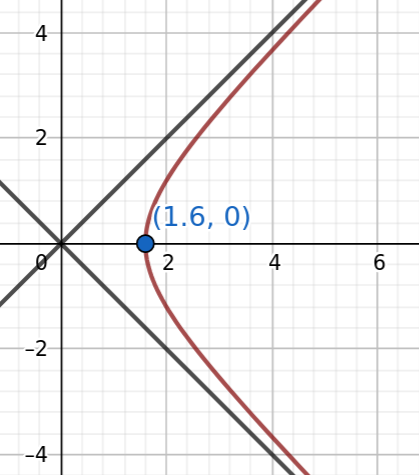
\includegraphics[width=60mm]{hiperbola1}
    \end{figure}

    Dibujar $\Phi(\theta_0,r)$ con $\theta_0$ fijo.

    Tenemos $x=r\ch\theta_0,\ y=r\sh\theta_0$ con $r\in\R^+$, que es
    la ecuación paramétrica de una semirecta que ``pasa'' (no llega a
    tocarlo porque $r>0$) por el origen. La pendiente será
    $\frac{y}{x}=\frac{\sh\theta_0}{\ch\theta_0}=\tanh\theta_0\in
    ]-1,1[$. Y la pendiente será mayor cuanto mayor sea $\theta_0$,
    puesto que $\tanh$ tiene esta forma:
    \begin{figure}[H] \centering
      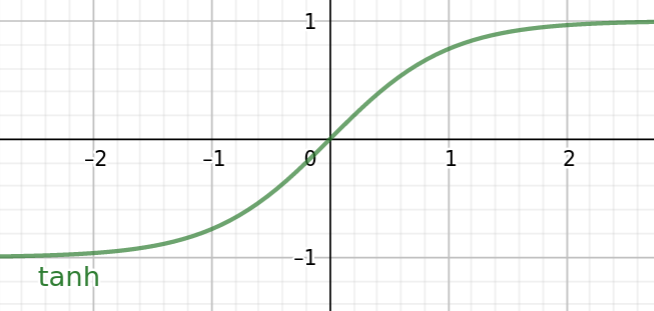
\includegraphics[width=80mm]{tanh}
    \end{figure}

    $\Phi(\theta_0,r)$ queda entonces de este modo (comparamos
    distintos valores de $\theta_0$).
    \begin{figure}[H] \centering
      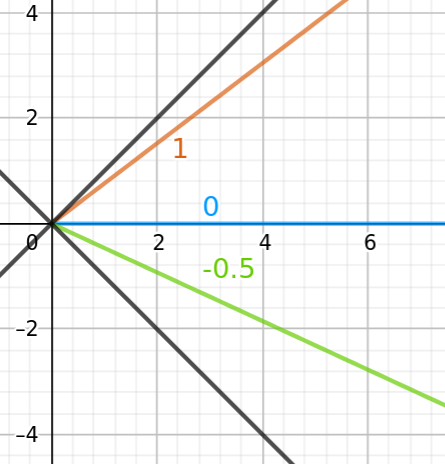
\includegraphics[width=60mm]{hiperbola2}
    \end{figure}

  \item Interpretar $\sh$ y $\ch$ en términos de ``trigonometría en la
    hipérbola''.

    Claramente $x=\ch\theta$ y $y=\sh\theta$ satisfacen la ecuación
    $x^2-y^2=1$. $y$ toma valores en todo $\R$ y $x$ a patir de $1$,
    luego $(\ch,\sh):\R\rightarrow\R^2$ parametriza la rama derecha de
    la hipérbola equilátera. Dado $A\in\R$, $(\ch A,\sh A)$
    corresponderá a un punto de dicha rama, y recíprocamente todo
    punto de la rama se escribe como $(\ch A,\sh A)$ para algún
    $A\in\R$. Para darle a $\sh$ y $\ch$ cierto carácter ``canónico''
    (¿Que tiene esta parametrización de la hipérbola de especial? ¿Por
    qué elegir ésta y no otra?) destacamos que el área azul de la
    figura es de $A$ unidades cuadradas.

    \begin{figure}[H] \centering
      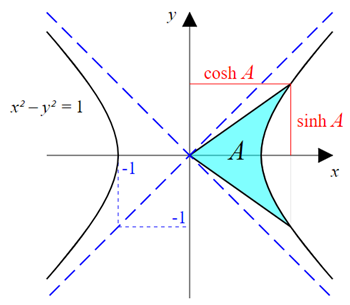
\includegraphics[width=80mm]{hiperbola3}
    \end{figure}

    Probaremos que el área azul por encima del eje vale $\frac{A}{2}$.
    El área bajo la recta $y=\frac{\sh A}{\ch A}x$ (que pasa por el
    origen y $(\ch A,\sh A)$) entre $0$ y $\ch A$ es
    \[\int_0^{\ch A} \frac{\sh A}{\ch A}xdx=\frac{\sh A}{\ch
        A}\Big[\frac{x^2}{2}\Big]_0^{\ch A}=\frac{\sh A\ch A}{2}\] Hay
    que restarle el área bajo la hipérbola ($y=\sqrt{x^2-1}$), que es
    \begin{align*}\int_1^{\ch A}\sqrt{x^2-1}dx&=\int_0^A\sqrt{\ch
                                                t^2-1}\sh t dt \qquad\text{(usando el cambio $x=\ch t$)} \\
                                              &=\int_0^A \sh^2t dt=\int_0^A \Big(\frac{e^t-e^{-t}}{2}\Big)^2 dt = \frac{1}{4}\int_0^A e^{2t}+e^{-2t}-2dt \\
                                              &=\frac{1}{4}\bigg(\Big[\frac{e^{2t}}{2}\Big]_0^A-\Big[\frac{e^{-2t}}{2}\Big]_0^A-\Big[2t\Big]_0^A\bigg) = \frac{1}{4}\bigg(\frac{e^{2A}}{2}-\frac{1}{2}-\Big(\frac{e^{-2A}}{2}-\frac{1}{2}\Big)-2A\bigg) \\
      &= -\frac{A}{2} +\frac{1}{4} \frac{e^{2A}-e^{-2A}}{2}
    \end{align*}

    Por tanto el área azul por encima del eje es
    \begin{align*}
      \frac{\sh A\ch A}{2} +\frac{A}{2} - \frac{1}{4} \frac{e^{2A}-e^{-2A}}{2} = \frac{A}{2} + \frac{1}{2}\frac{(e^A-e^{-A})}{2}\frac{(e^A+e^{-A})}{2}-\frac{1}{4}\frac{e^{2A}-e^{-2A}}{2}=\frac{A}{2}
    \end{align*}
  \end{enumerate}
\end{exercise}

\newcommand{\T}{T_1(\mathbb{S}^2)}
\newcommand{\E}{\mathcal{E}_*(e)}

\newpage
\begin{exercise}

  Se considera el grupo el grupo de rotaciones
  \[SO(3)=\{A\in\R^{3\times 3}:A^T A=AA^T=I,\ \det A>0\}\]

  \begin{enumerate}[a)]
  \item Probar que la aplicación
    \[\Phi:SO(3)\rightarrow \T=\{(x,y)\in\R^3\times\R^3:|x|=|y|=1,\
      <x,y>=0\}\] que a cada matriz $A\in SO(3)$ le hace corresponder
    sus dos primeras columnas es un homeomorfismo.

    Dada una matriz $A=(a_1|a_2|a_3)$, tenemos que $A$ es ortogonal
    ($A^T A=AA^T=I$) si, y solo si $(a_1,a_2,a_3)$ forma una base
    ortonormal de $\R^3$; y $\det A>0$ si, y solo si la base define
    una orientación positiva (como los vectores son ortonormales, esto
    equivale a que $a_1\times a_2=a_3$). Por tanto si $A\in SO(3)$,
    sus dos primeras columnas son ortonormales: $(a_1,a_2)\in\T$, así
    que $\Phi$ está bien definida.

    ¿Es biyectiva? De existir $\Phi^{-1}$, tendría que ser de esta
    forma: para $(x,y)\in\T$, \\ $\Phi^{-1}(x,y)=A=(x|y|z)$. Para que
    esto sea una aplicación bien definida, tiene que existir un único
    $z$ que haga que $A$ sea ortogonal y preserve la orientación
    (tenga determinante positivo). $(x,y,z)$ será una base ortonormal
    si, y solo si $z\bot x,y$ y $|z|=1$. Lo primero implica que
    $z\in \operatorname{Lin}\{x,y\}^\bot$, que es una recta, así que
    sólo hay dos posibilidades para $z$, $z=\pm x\times y$. Pero sólo
    $z=+x\times y$ hace que la orientación de la base ortonormal
    sea positiva ($\det A>0$). Por tanto $\Phi$ es biyectiva con \\
    $\Phi^{-1}(x,y)=(x|y|x\times y)$.

    Claramente $\Phi$ es continua por ser la restricción a $SO(3)$ de
    la proyección de $\R^{3\times 3}$ a $\R^{3\times 2}$. Y
    $\Phi^{-1}$ lo es por serlo el producto vectorial (consecuencia de
    $|(x-u)\times (y-v)|$\\
    $=|x-u||y-v|\sin(\sphericalangle(x-u,y-v))\leq |x-u||y-v|$), luego
    $\Phi$ homeomorfismo.

  \item $e\in]0,1[$, $\E$ espacio de órbitas keplerianas con
    excentricidad $e$. Es decir, el conjunto de pares $(V,E)$ con
    $V\subset\R^3$ plano vectorial orientado y $E\subset V$ elipse con
    foco en el origen y excentricidad $e$. Probar que existe una
    biyección entre $\E$ y $SO(3)\times\R^+$.

    Probamos algo equivalente: encontramos una biyección entre $\E$ y
    $\T\times\R^+$, ya que sabemos que $SO(3)$ es biyectivo con $\T$.

    Dado $\big((x,y),r\big)\in\T\times\R^+$, le hacemos corresponder
    el plano vectorial $V=x^\bot$ orientado con la orientación
    inducida por cualquier base $\{v_1,v_2\}$ de $V$ que convierta a
    $(v_1,v_2,x)$ en una base positivamente orientada de $\R^3$, esto
    es: $\det(v_1,v_2,x)>0$.

    Para que esta definición sea correcta, debemos comprobar que la
    orientación de $V$ no depende de la base escogida. En efecto, si
    $(v_1,v_2)$ y $(u_1,u_2)$ son dos bases de $V$ que cumplen
    $\det(v_1,v_2,x), \det(u_1,u_2,x)>0$, escribimos $v_1$ y $v_2$ en
    función de $(u_1,u_2)$,
    \[v_1=a_{11}u_1+a_{12}u_2,\qquad v_2=a_{21}u_1+a_{22}u_2\] La
    matriz de cambio de base $(v_1,v_2)$ a $(u_1,u_2)$ es
    \[M=\begin{pmatrix}
        a_{11} & a_{21} \\
        a_{12} & a_{22}
      \end{pmatrix}\] para probar que ambas bases definen la misma
    orientación en $V$ debemos comprobar que
    $\det M=a_{11}a_{22}-a_{21}a_{12}>0$. Usaremos para ello
    propiedades básicas de los determinantes.
    \begin{align*}
      \det(v_1,v_2,x)=\det(a_{11}u_1&+a_{12}u_2,a_{21}u_1+a_{22}u_2,x) \\
       =\det(a_{11}u_1,a_{21}u_1+a_{22}u_2,x)&+\det(a_{12}u_2,a_{21}u_1+a_{22}u_2,x) \\
      =\det(a_{11}u_1,a_{21}u_1,x)+\det(a_{11}u_1,a_{22}u_2,x)&+\det(a_{12}u_2,a_{21}u_1,x)+\det(a_{12}u_2,a_{22}u_2,x) \\
      =a_{11}a_{21}\det(u_1,u_1,x)+a_{11}a_{22}\det(u_1,u_2,x)&+a_{12}a_{21}\det(u_2,u_1,x)+a_{12}a_{22}\det(u_2,u_2,x) \\
      =a_{11}a_{22}\det(u_1,u_2,x)&+a_{12}a_{21}\det(u_2,u_1,x) \\
      =a_{11}a_{22}\det(u_1,u_2,x)&-a_{12}a_{21}\det(u_1,u_2,x) \\
      =(a_{11}a_{22}-a_{12}a_{21})&\det(u_1,u_2,x) = \det M \det(u_1,u_2,x)
    \end{align*}
    Por tanto $\det M>0$ y probamos que esta correspondencia está bien
    definida.

    Como $(x,y)\in \T$, $y\bot x\Rightarrow y\in x^\bot = V$, lo que
    nos permite usar $y$ como sentido para el eje de excentricidad de
    la elipse. $E$ será por tanto la elipse con parámetros $k=r$ y
    $\vec{e}=ey$.

    Recíprocamente, dado $(V,E)\in \E$ le hacemos corresponder
    $\big((x,y),r\big)$, donde $x$ será el vector unitario normal al
    plano $V$ (hay dos posibilidades, un vector y su opuesto) que
    respete la orientación en $V$, es decir, si $(v_1,v_2)$ es una
    base de $V$, $x$ será el vector unitario que cumple
    $x=\lambda\cdot v_1\times v_2$ con $\lambda >0$, o
    equivalentemente $\det(v_1,v_2,x)>0$. Los argumentos anteriores
    también prueban que dos bases de $V$ que definan la misma
    orientación dan luegar al mismo $x$ (puesto que $\det M>0$).

    $y\in V$ será el vector unitario con el sentido del eje de
    excentricidad de $E$: $y=\dfrac{\vec{e}}{e}$. Como $x\in V^\bot$,
    tendremos $x\bot y$ y por tanto $(x,y)\in\T$. Finalmente, tomamos
    $r=k\in\R^+$, el parámetro de $E$.

    Estas correspondencias son una inversa de la otra: $x$ y $V$
    (respectivamente $y$ y $\vec{e}$; y \\ $r$ y $k$) se definen
    unívocamente.

  \item Caso $e=0$.

    Ahora $\E$ está formado por circunferencias en planos orientados.

    Las correspondencias entre $x$ y $V$ (plano orientado en el que
    está la circunferencia); y entre $r$ y $k$ (radio de la
    circunferencia) siguen siendo válidas. Pero $\vec{e}=0$
    independientemente de $y\in x^\bot = V$, luego la correspondencia
    anterior ya no es una biyección. Esto no descarta que exista otra
    biyección, probablemente la haya, aunque no sea tan fácil de
    interpretar.
  \end{enumerate}
\end{exercise}

\newpage
\setcounter{exercise}{10}
\begin{exercise}
  Dado un campo $C^\infty$,
  $V=(V_1,V_2):\mathbb{R}^2\rightarrow\mathbb{R}^2$ cumpliendo
  $\operatorname{div}V=\frac{\partial V_1}{\partial x}+\frac{\partial
    V_2}{\partial y}=1$, debemos encontrar $F\in C^\infty(\mathbb{R}^2)$
  tal que
  \begin{equation} \label{eq:V}
    V=J\nabla F+V_*=\left(-\frac{\partial F}{\partial y},\frac{\partial F}{\partial x}\right)+V_*
  \end{equation} 
  donde $V_*:\mathbb{R}^2\rightarrow\mathbb{R}^2$ es fijo.

  Dado $V$, supondremos que se puede expresar como en (\ref{eq:V})
  para obtener condiciones sobre $F$ y $V_*$. Con estas condiciones
  obtendremos candidatos a $F$ y $V_*$, para después comprobar que
  efectivamente $V$ se puede expresar de esa forma.

  Tomando divergencias en (\ref{eq:V}) y utilizando que la divergencia
es un operador lineal, obtenemos
\[1=\operatorname{div}V = -\frac{\partial^2 F}{\partial x\partial
    y}+\frac{\partial^2 F}{\partial y\partial
    x}+\operatorname{div}V_*\] Utilizando que
$\dfrac{\partial^2 F}{\partial x\partial y}=\dfrac{\partial^2
  F}{\partial y\partial x}$, obtenemos
$\operatorname{div}V_*=1$. Observamos que si se cumpliese (\ref{eq:V})
para un $V_*$, existiría una $F_0$ tal que el campo
$V_0(x,y)=(\frac{x}{2},\frac{y}{2})$, que tiene divergencia 1, se
expresase como
$V_0=\left(-\frac{\partial F_0}{\partial y},\frac{\partial
    F_0}{\partial x}\right)+V_*$. Por otra parte, dado cualquier $V$
con divergencia 1, existiría $F$ tal que
$V=\left(-\frac{\partial F}{\partial y},\frac{\partial F}{\partial
    x}\right)+V_*$. Obtendríamos por tanto
\[V=\left(-\frac{\partial F}{\partial y},\frac{\partial F}{\partial
      x}\right)+V_0-\left(-\frac{\partial F_0}{\partial
      y},\frac{\partial F_0}{\partial x}\right)=\left(-\frac{\partial
      (F-F_0)}{\partial y},\frac{\partial (F-F_0)}{\partial
      x}\right)+V_0\] Con esto hemos demostrado que no importa el
$V_*$ que tomemos, ya que sólo hará que varíe la función $F$, pero no
afectará a su existencia. Tomamos por tanto
$V_*=V_0=(\frac{x}{2},\frac{y}{2})$.

Discutamos ahora $F$. Dado $V=(V_1,V_2)$ con $\operatorname{div}V=1$,
(\ref{eq:V}) nos proporciona un sistema de ecuaciones en derivadas
parciales que tiene que cumplir $F$.
\begin{align} 
   V_1&=-\frac{\partial F}{\partial y}+\frac{x}{2} \label{eq:dy}\\
   V_2&=\frac{\partial F}{\partial x}+\frac{y}{2} \label{eq:dx}
\end{align}

La existencia de $F$ dependerá de la existencia de solución para este
sistema.

Tomando primitivas respecto de $y$ en (\ref{eq:dy}) obtenemos:
\begin{equation} \label{eq:Fc}
  F(x,y)=\frac{xy}{2}-\int_0^y V_1(x,s)ds+c(x),
\end{equation}
ya que al tomar primitivas respecto de $y$ nos aparece una constante
que puede depender de $x$ (constante respecto de $y$). Para determinar
$F$, falta determinar $c(x)$, ya que el resto de sumandos son
conocidos.

Considerando $y\in\mathbb{R}$ fijo,
$c:\mathbb{R}\rightarrow\mathbb{R}$ viene dada por
$c(x)=F(x,y)-\frac{xy}{2}+\int_0^y V_1(x,s)ds$. Utilizando el Teorema
de Derivación Bajo el Signo Integral, obtenemos que
$c\in C^1(\mathbb{R})$ y se cumple:
\[\frac{\partial F}{\partial x}(x,y)=\frac{y}{2}-\int_0^y
  \frac{\partial V_1}{\partial x}(x,s)ds+c'(x)\] Notemos que en
(\ref{eq:V}) sólo aparece el gradiente de $F$, por lo que debemos
determinar $F$ salvo constante. Así que nos basta con determinar
$c'(x)$. Igualamos está ecuación con (\ref{eq:dx}):
\begin{equation} \label{eq:V2}
  V_2(x,y)-\frac{y}{2}=\frac{y}{2}-\int_0^y
  \frac{\partial V_1}{\partial x}(x,s)ds+c'(x)
\end{equation}

Primero resolveremos la integral, aplicando
$\frac{\partial V_1}{\partial x}+\frac{\partial V_2}{\partial y}=1$ y
utilizando la regla de Barrow:
\begin{equation} \label{eq:int}
  \int_0^y \frac{\partial V_1}{\partial x}(x,s)ds=\int_0^y
  1-\frac{\partial V_2}{\partial y}(x,s)ds=y-\big(V_2(x,y)-V_2(x,0)\big)
\end{equation}
Sustituimos en (\ref{eq:V2}):
\begin{equation} \label{eq:c'}
  V_2(x,y)-\frac{y}{2}=\frac{y}{2}-y+V_2(x,y)-V_2(x,0)+c'(x)
\end{equation}
Simplificando $V_2$ e $y$, obtenemos $c'(x)=V_2(x,0)$ y tomamos
$c(x)=\int_0^x V_2(t,0)dt$.

Recuperando (\ref{eq:Fc}), obtenemos finalmente:
\begin{equation}
  \label{eq:F}
  F(x,y)=\frac{xy}{2}-\int_0^y V_1(x,s)ds+\int_0^x V_2(t,0)dt
\end{equation}
Utilizando el Teorema Fundamental del Cálculo, obtenemos que
$\frac{\partial F}{\partial y}$ existe y es continua en todo
$\mathbb{R}^2$, mientras que combinando el Teorema de Derivación Bajo
el Signo Integral con el Teorema Fundamental del Cálculo, deducimos
que $\frac{\partial F}{\partial x}$ existe y es continua en todo
$\mathbb{R}^2$. Por tanto, $F$ es $C^1(\mathbb{R}^2)$. Comprobamos
ahora que efectivamente se cumple (\ref{eq:V}) obteniendo las derivadas parciales de $F$:
\begin{equation*}
  \left(-\frac{\partial F}{\partial y},\frac{\partial F}{\partial x}\right)=\left(-\frac{x}{2}+V_1(x,y),\frac{y}{2}-\int_0^y \frac{\partial V_1}{\partial x}(x,s)ds+V_2(x,0)\right)
\end{equation*}
Volvemos a utilizar $\operatorname{div}V=1$ y la regla de Barrow para
calcular el valor de la integral como en (\ref{eq:int}), y
simplificamos:
\begin{align*}
  \left(-\frac{\partial F}{\partial y},\frac{\partial F}{\partial x}\right)&=\left(-\frac{x}{2}+V_1(x,y),\frac{y}{2}-y+V_2(x,y)-V_2(x,0)+V_2(x,0)\right) \\
  &=\left(-\frac{x}{2}+V_1(x,y),-\frac{y}{2}+V_2(x,y)\right)=V-V_*
\end{align*}
Viendo ahora que las derivadas parciales de $F$ son
$C^\infty(\mathbb{R^2})$, concluimos que $F\in C^\infty(\mathbb{R}^2)$.
\end{exercise}

\end{document}
